Para crear un Issue desde terminal es fácil primero tenemos que tener git en consola primero debemos de estar en un repositorio con colaboradores y clonar el repositorio remoto en uno local cree un archivo python con un error simulando un producto de un proyecto en consola lo primero que hice fue a agregar al repositorio local con un git add y git commit despues de 
eso cargue al repositorio remoto con un git push  cree un Isseu utilizando el comando gh issue create donde le puse un titulo despues asigne a mi compañero luis como responsable de corregir el error asi tambien liste a mi compañero debido a que me equivo al poner el numero de issue intente ponerle una etiqueta pero no pude haci que le puse una que decia chinita su amor platonico de mi compañero.



\begin{figure}[H]
    \centering
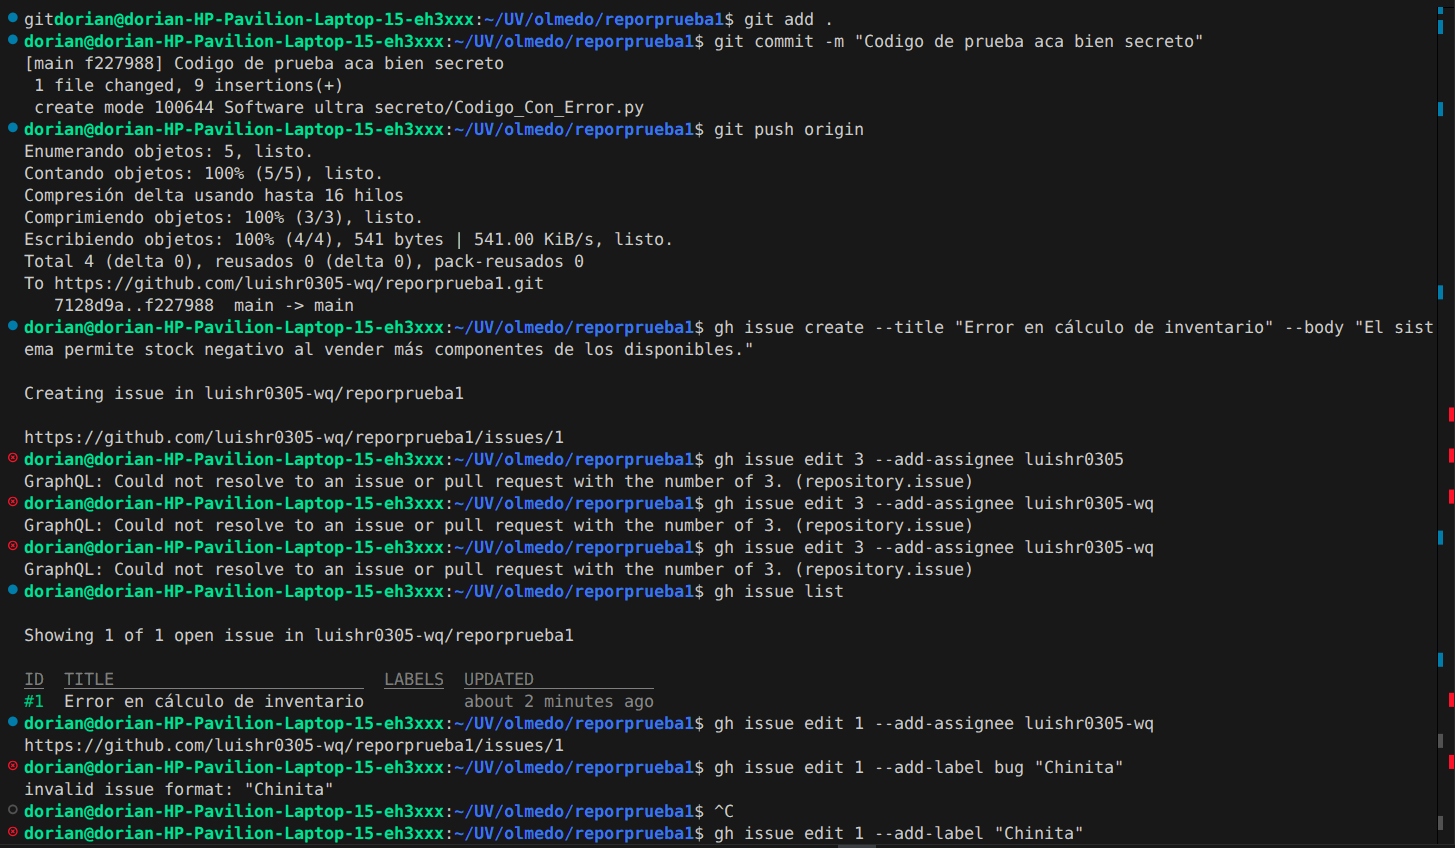
\includegraphics[width=1\textwidth]{imagenes/issuecli.png}
    \caption{creación de Issue}
    \label{fig:Dc1}
\end{figure}


\begin{figure}[H]
    \centering
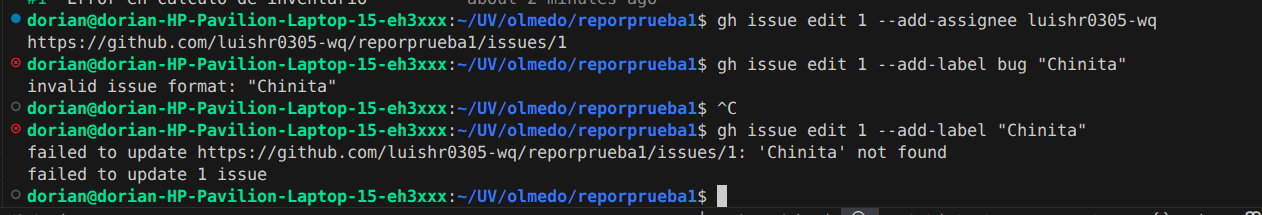
\includegraphics[width=1\textwidth]{imagenes/issue2cli.png}
    \caption{Asignación a issue y etiqueta del mismo}
    \label{fig:Dc2}
\end{figure}

Bueno aqui lo que hace mi compañero es bajar el repositorio con un git clone debido a que lo inicializo en la nube y no tenia archivos ahi despues ingreso a la carpeta donde se encontraba el repositorio y el archivo con error despues de arreglar el error hizo un git add . y despues un commit para posteriormente subirlo al repositorio remoto ya por ultimo cerro el isseu con un git issue close id de el issue 


\begin{figure}[H]
    \centering
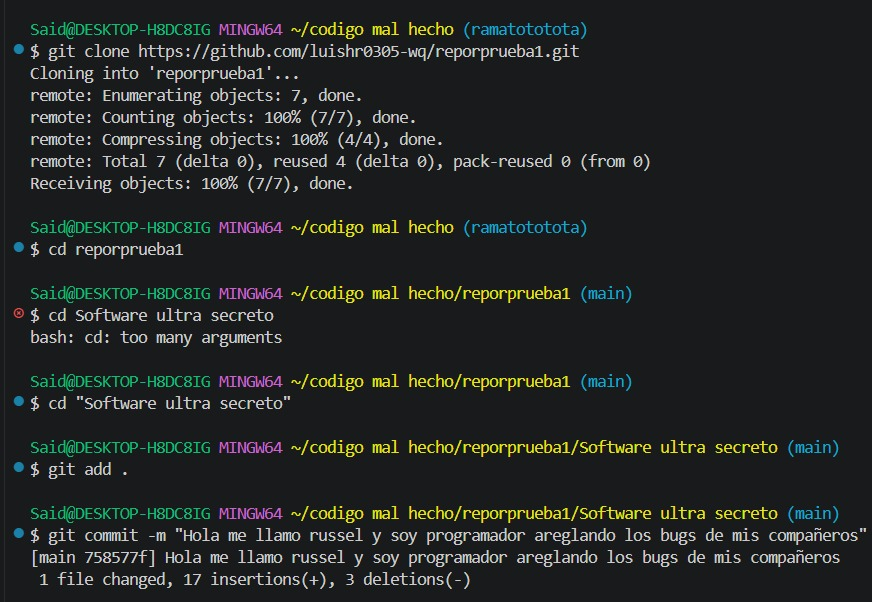
\includegraphics[width=1\textwidth]{imagenes/issue3.jpeg}
    \caption{}
    \label{fig:Dc3}
\end{figure}
